\chapter{Vorhandene Glücksspielseiten}
\section{Bitcoin}
Die Internetseite Crypto Games \cite{crypto_games} bietet ein Würfelspiele an, bei dem der Nutzer mit Kryptowährungen bezahlen kann. Der Spieler wettet darauf, dass der Wert einer ''zufällig'' generierten Zahl liegt zwischen 0 und 100 über einem bestimmten Zielwert liegt. Der Spieler kann nachdem die Wette platziert ist eigenständig prüfen, ob er gewonnen oder verloren hat.
\begin{figure}[H]
\centering
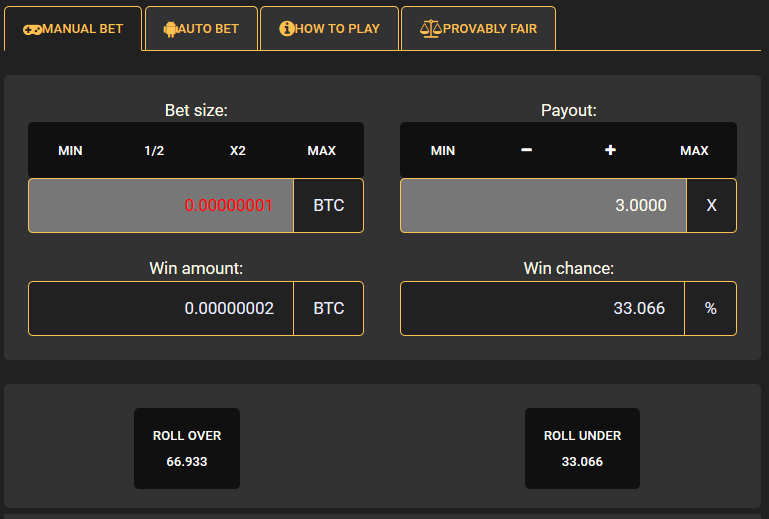
\includegraphics[scale=0.5]{Figures/crypto_games}
\decoRule
\caption{MANUAL BET}
\label{fig:crypto_games}
\end{figure}

Das Formular aus Abbildung \ref{fig:crypto_games} lässt den Spieler die Höhe des Einsatz und den Multiplikator anpassen. Je höher der Multiplikator, desto höher passt die Glücksspielseite den Zielwert an.

Bereits bevor der Spieler die Wette abschließt, teilt ihm die Seite den SHA256 Hash des sogenannten ''Server seed'' mit. Der Server Seed ist zu diesem Zeitpunkt nur dem Service bekannten und wird erst nach dem Abschluss der Wette veröffentlicht.
Außerdem ermöglicht die Seite es dem Spieler den sogenannten ''Next client seed'' frei zu wählen. Dieser geht zusammen mit dem Server Seed in die Berechnung der Gewinnerauswahl ein. Sobald der Spieler die Wette abschließt, veröffentlicht der Service den ''Server seed''. Der Spieler kann durch die Berechnung des SHA256 Hash nachprüfen, ob es sich wirklich um den echten Wert handelt.

\begin{figure}[H]
\centering
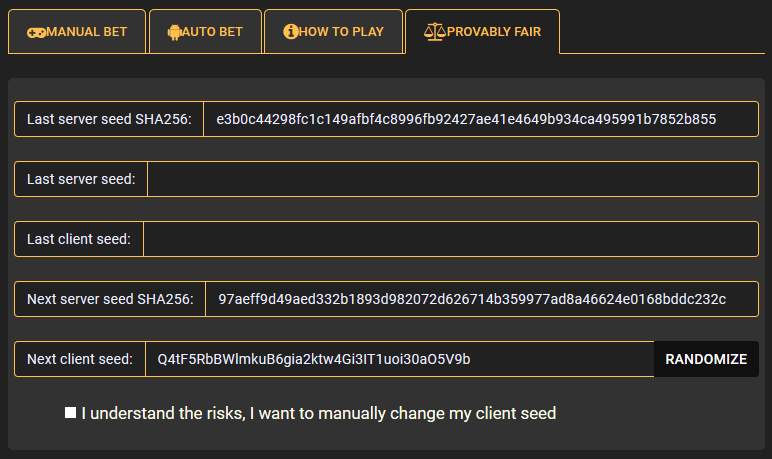
\includegraphics[scale=0.5]{Figures/crypto_games_details}
\decoRule
\caption{PROVABLY FAIR}
\label{fig:crypto_games_details}
\end{figure}

Nun erfolgt die Gewinnerauswahl. Zunächst wird der SHA512 Hash des konkatenierten Server und Client Seeds berechnet. Dieser Hash Wert liefert die Zufallsquelle für die Gewinnerauswahl. Die ersten 5 Stellen des Hashs in Hexadezimaldarstellung werden in eine Dezimalzahl konvertiert. Anschließend werden die letzten 5 Ziffern als Zahl zwischen 0 und 100 mit 3 Nachkommastellen betrachtet. Die nachfolgende Abbildung veranschaulicht diesen Prozess.

\begin{figure}[H]
\centering
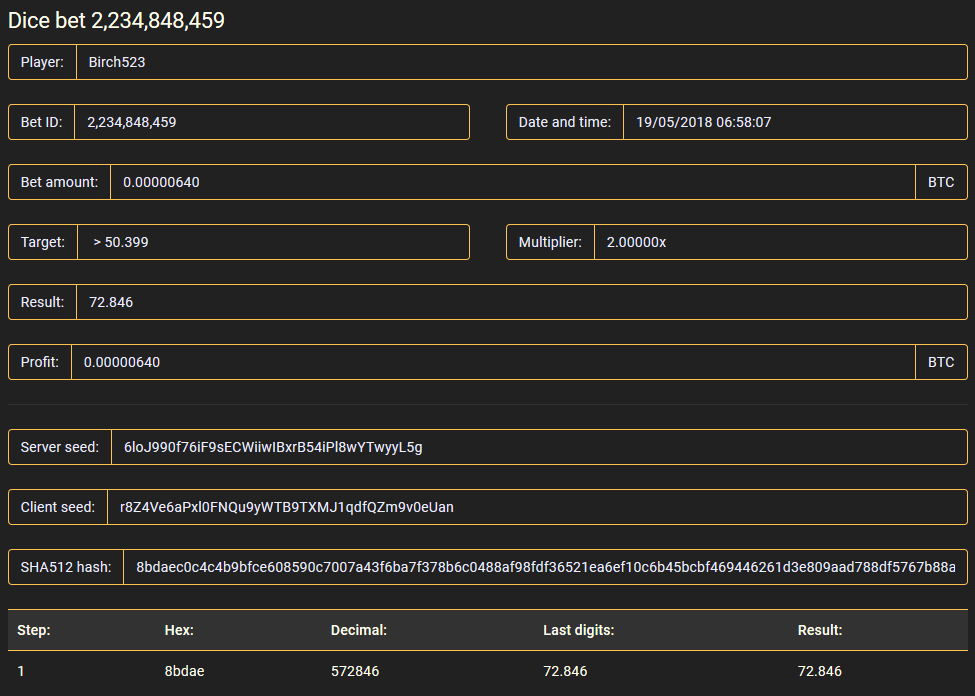
\includegraphics[scale=0.5]{Figures/crypto_games_result}
\decoRule
\caption{BET RESULT}
\label{fig:crypto_games_result}
\end{figure}

Im Beispiel aus Abbildung \ref{fig:crypto_games_result} liegt die resultierende Zahl (72,846) über dem Zielwert 50,399. Dies führt dazu, dass der Spieler gewinnt und seinen Einsatz ausgezahlt bekommt.

\section{Ethereum}

Die Internetseite \cite{vdice} bietet ein Würfelspiel an, das durch einen Smart Contract auf der Ethereum Plattform umgesetzt ist. Die Internetseite übernimmt dabei lediglich die Visualisierung der platzierten Wetten. Die Teilnahme benötigt keinen Account, da man ausschließlich mit dem Smart Contract\footnote{\url{https://etherscan.io/address/0xdd98b423dc61a756e1070de151b1485425505954\#code}} interagiert. Statt des Blockhashs wird ein sogenannter Oracle Service \cite{oracalize_it} zur Gewinnerauswahl verwendet. Dieser liefert Zufallszahlen des Services \cite{random_org} zusammen mit einer eine Echtheitsgarantie (Signatur) innerhalb von Transaktionen an den Smart Contract. Der Smart Contract prüft die Echtheit der Daten mittels der Signatur und führt anschließend die Gewinnerauswahl und Auszahlung durch. Detaillierte Informationen über die Funktionsweise eines Oracles und dessen Einsatzmöglichkeiten findet man unter \cite{eth_oracles}.